\documentclass[border=10pt]{standalone}
\usepackage{pgfplots}
\pgfplotsset{compat=1.18}
\begin{document}
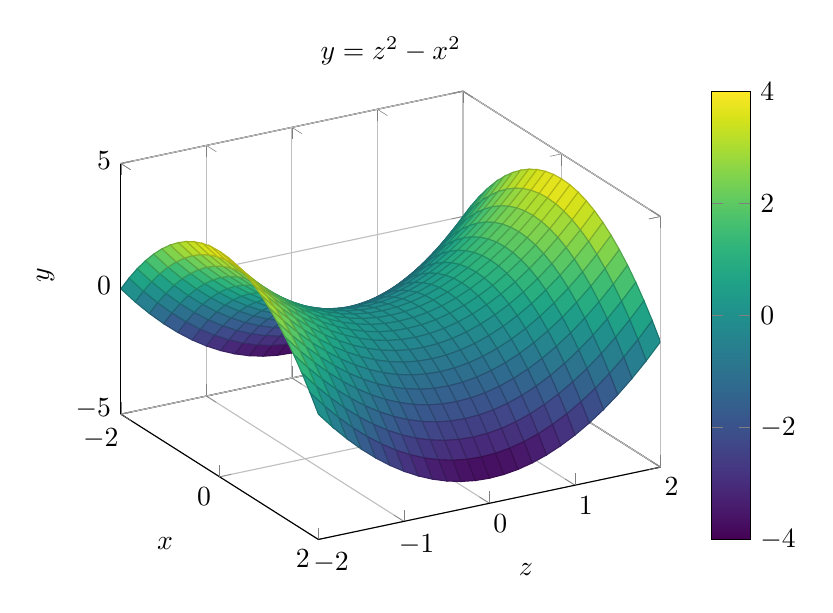
\begin{tikzpicture}
\begin{axis}[
    view={60}{30},
    xlabel={$x$},
    ylabel={$z$},
    zlabel={$y$},
    title={$y = z^2 - x^2$},
    domain=-2:2,
    y domain=-2:2,
    samples=25,
    colormap/viridis,
    colorbar,
    grid=major,
    zmin=-5,
    zmax=5
]
% Map: x_plot = x, y_plot = z, z_plot = y = z^2 - x^2 = y_plot^2 - x_plot^2
\addplot3[surf] {y^2 - x^2};
\end{axis}
\end{tikzpicture}
\end{document}